\documentclass[12pt,a4paper]{article}
%\renewcommand{\familydefault}{\ttdefault}
\pagenumbering{gobble} %remove page number
\usepackage[font=small,labelfont=bf]{caption} % Required for specifying captions to tables and figures
\usepackage{lmodern} %to fight font errors
\usepackage{array,booktabs,ragged2e}%centering tables 
\usepackage{polski}
\usepackage[utf8]{inputenc} 
\usepackage{blindtext}
\usepackage{longtable}
\usepackage[left=1.0cm,right=1.0cm,top=1cm,bottom=0.0cm]{geometry}
\usepackage{multirow}
\usepackage{verbatim}
\usepackage{multicol}
\setlength\columnsep{-6.0cm} % This is the default columnsep for all pages
\usepackage{tabularray}
\usepackage{graphicx}
\usepackage{hyperref}
\usepackage{indentfirst} % indent first paragraph
\usepackage{enumitem} %[leftmargin=*]

\hypersetup{colorlinks=true,linkcolor=blue,urlcolor=blue}

\usepackage{color}
\definecolor{techColor}{RGB}{120, 120, 120}

\begin{document}

\begin{tabular}  { >{\RaggedLeft} p{16cm}  p{3cm} }  
	{\Large \textbf{KRZYSZTOF BOBNIS}} \hfill Wrocław & \textcolor{techColor}{residence} \\
	 GAME PROGRAMMER, GAME JAMMER \hfill  {\href{mailto:kbobnis@gmail.com}{kbobnis@gmail.com}} & \textcolor{techColor}{email} \\ 
	 \hfill {\href{https://www.linkedin.com/in/krzysztofbobnis}{linkedin.com/in/krzysztofbobnis}} & \textcolor{techColor}{linkedin} \\
	 \hfill {\href{http://bobnis.eu}{bobnis.eu}} & \textcolor{techColor}{portfolio} \\
\end{tabular}	 

\vspace{1cm}

\begin{multicols}{2}


\centering
\section*{Summary}
\justifying
	\noindent Graduated from Wrocław University of Technology with AI and advanced computer graphics specialties. My thesis was based on fractal structures and genetic algorithms. During that time we learned c++ and wrote many experimental programs in it. Worked in Canada for 2 years on AR and video streaming based games. \\

	\textbf{Experience}: Programmer with 11 years of experience (8 years of experience with shipped games).
	
	\textbf{Excellent with}: Unity3d, c\#, php, google play store, git, svn, communication, english, game design, UX.
	
	\textbf{Very good with}: C++, java (native android), as3, app store, algebra, AI, computer graphics.

\begin{samepage}
\centering
\section*{Experience }
\justifying

	\textbf{Tech Lead} / 2020 - Present
		{\href{https://dali.games/}{Dali Games}} - Created scriptless adventure game tool for unity. This codebase was used to create two games: {\href{https://play.google.com/store/apps/details?id=games.dali.adventure.neighborhood.unholy}{Unholy}} 100,000+ installs and {\href{https://play.google.com/store/apps/details?id=games.dali.adventure.reborn}{Reborn}} 100,000+ installs. 

	\textbf{Senior Game Programmer} / 2018 - 2020\\
		{\href{https://cat-astrophe-games.com/}{Cat-astrophe Games}} - Created working prototype of run / walk / steps verifier as a game on a mobile phone. \\
		{\href{https://www.uken.com/}{Uken}}, Toronto, Canada  - Worked on a live video streaming game prototype with user interaction. Also developed game {\href{https://play.google.com/store/apps/details?id=com.uken.pool}{Kings of Pool }} with  500,000+ installs. 

	\textbf{Game Programmer} / 2012 - 2017\\ 
		{\href{https://tensquaregames.com/}{TSG}}, {\href{https://www.uken.com/}{Uken}} - Learned and applied frontend and backend technologies in as3, php, java, c\#, redis, mysql, git, svn to free to play web and mobile platforms. Game I was developing: {\href{https://play.google.com/store/apps/details?id=air.com.tensquaregames.letsfish}{Lets-Fish}} has 10,000,000+ installs.

	\textbf{Student} / 2006 - 2011 \\
		Graduated with Master of Science, Information Technology on Wroclaw University of Technology, Major: Computer Science. Educational profiles: Artificial Intelligence, Advanced Computer Graphics, Computer Networks. \\

\end{samepage}

\vfill 



\begin{itemize}[leftmargin=7.0cm]
	\centering
	\section*{Works}
	\justifying
	\setlength\itemsep{0.0cm}
	\item[] \textbf{C++ / SFML / STL} / 2022: \\
		Created a tetris game {\href{https://github.com/kbobnis/tetris}{Tetris - Github}}
	\item[] \textbf{Practical codebase} / 2021: \\
		Created and maintained an adventure creator tool used in two games {\href{https://play.google.com/store/apps/details?id=games.dali.adventure.neighborhood.unholy}{[1]}}, {\href{https://play.google.com/store/apps/details?id=games.dali.adventure.reborn}{[2]}}
	\item[] \textbf{Unreal game prototype} / 2017  \\
		 Created on a game jam  {\href{https://github.com/kbobnis/2017.05-TSG-Compo---Dead-eye}{Dead eye - Github}}
	\item[] \textbf{Won Game Jam} / 2016   \\
		1st place on TK Game Jam: {\href{https://itch.io/jam/tk-game-jam-2016/results}{itch.io}} 
	\item[] \textbf{Self publisher} / 2015 \\
		 My game made US\$10,000+: {\href{https://play.google.com/store/apps/details?id=com.wyspianStudios.rpgModuleFull}{RPG Module}} 
\end{itemize}


\begin{itemize}[leftmargin=7.0cm]
	\centering	
	\section*{Languages }
	\justifying
	\setlength\itemsep{0.0cm}
	\item[] \textbf{English} - \textbf{fluent}: relocated for 2 years to work as a game programmer in Toronto, Canada, passed ACERT: C1 english certificate.
	\item[] \textbf{Polish} - \textbf{native}: born and lives in Wroclaw.
\end{itemize} 

\vfill

\end{multicols}

\vfill

Some of my game jam entries (all are listed on my portfolio {\href{http://www.bobnis.eu}{http://www.bobnis.eu}}):
\begin{table}[htbp]
    \centering
    \begin{tblr}{colspec={X X X X X X }, row{1} = {c}}
		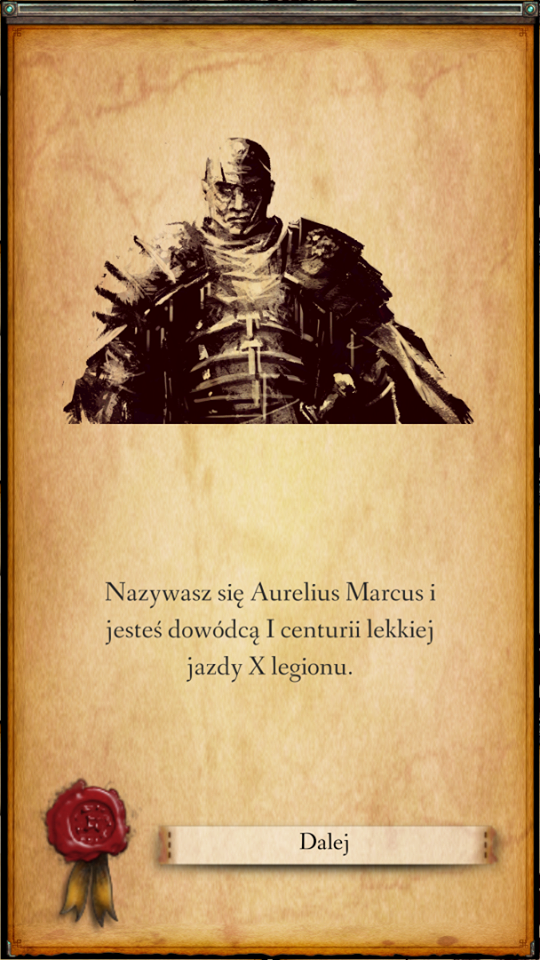
\includegraphics[height=3.0cm,width=1.75cm]{games/rpg_module2.png}
		&  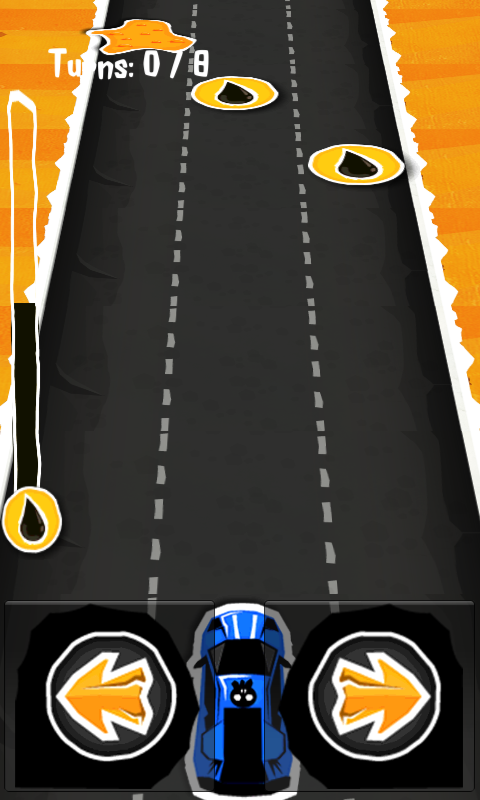
\includegraphics[height=3.0cm,width=1.75cm]{games/zcs.png}
		& 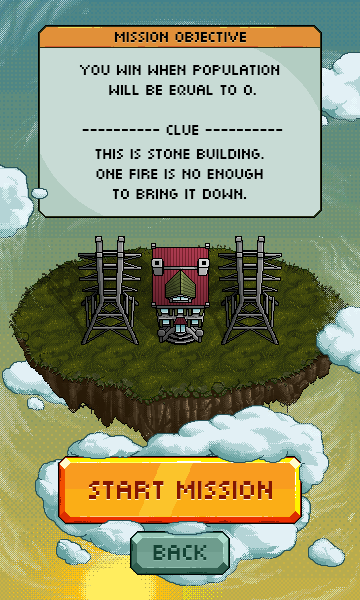
\includegraphics[height=3.0cm,width=1.75cm]{games/fog.png}
		& 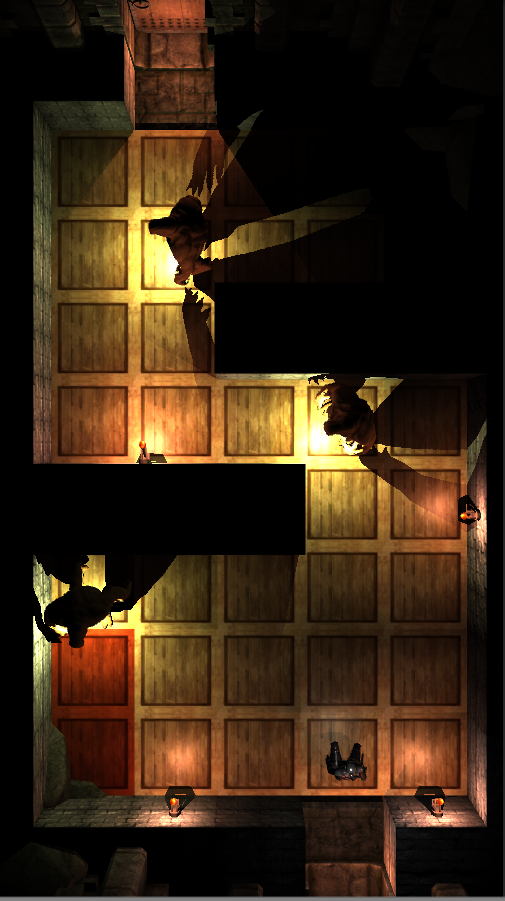
\includegraphics[height=3.0cm,width=1.75cm]{games/stealthRpg.png} 
		& 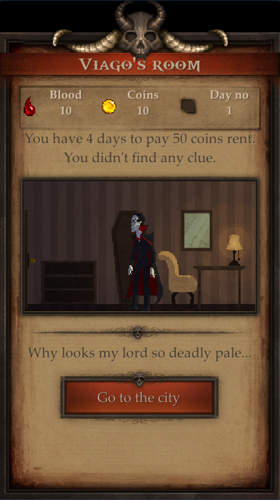
\includegraphics[height=3.0cm,width=1.75cm]{games/viago1.png} 
		&  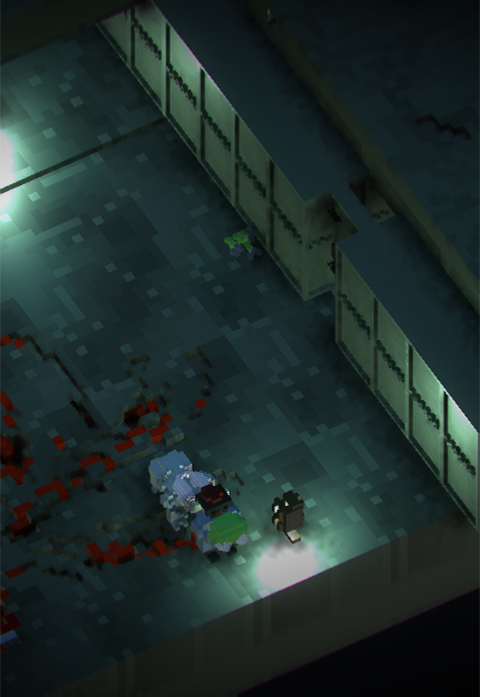
\includegraphics[height=3.0cm,width=1.75cm]{games/scp.png} \\

		  \centering RPG Module
		& \centering Zombie car smasher
		& \centering Finger of God
		& \centering Stealth RPG
		& \centering Viago the Vampire
		& \centering SCP-35
    \end{tblr}
\end{table}


\end{document}
